
\chapter{Einleitung}

Die Implementierung von E-Bikes erfuhr in den vergangenen Jahren eine bemerkenswerte Entwicklung, die nicht nur das Mobilitätsverhalten beeinflusste, sondern auch neue Perspektiven für nachhaltige Fortbewegung eröffnete.
Angesichts der drängenden Herausforderungen der Verkehrswende erweisen sich E-Bikes als vielversprechende Alternative zu herkömmlichen Verkehrsmitteln.\\

Um ein fundiertes Verständnis dieses Fachgebiets zu erlangen und ein individuell angepasstes und voll funktionsfähiges E-Bike zu entwickeln, wurde dieses Thema als Gegenstand meiner Studienarbeit gewählt.
Die Studie zielt darauf ab, die verschiedenen Aspekte der E-Bike-Technologie zu erforschen und eine maßgeschneiderte Lösung zu entwickeln, die den individuellen Bedürfnissen und Anforderungen gerecht wird.\\

Die Komplexität der verschiedenen Komponenten eines E-Bikes erfordert eine gründliche Analyse und Planung.
Besondere Herausforderungen ergeben sich beispielsweise bei der Integration von selbstgebauten Batterien in maßgeschneiderte E-Bikes.
Diese Batterien müssen nicht nur den Energiebedarf des E-Bike-Motors effizient decken, sondern auch den hohen Sicherheits- und Zuverlässigkeitsstandards entsprechen.\\

Das erwartete Ergebnis dieser Studienarbeit ist ein voll funktionsfähiges, selbstgebautes E-Bike, welches den individuellen Anforderungen und Vorlieben des Fahrers entspricht.
Durch eine gründliche Analyse und Implementierung aller relevanten Komponenten wird angestrebt, ein E-Bike zu entwickeln, das nicht nur effizient und zuverlässig ist, sondern auch einen Beitrag zur Mobilität leistet.\\

Angesichts der Vielzahl an Komponenten, aus denen ein E-Bike besteht, wurden für die Untersuchungen, das Design und die Implementierung folgende Schwerpunkte festgelegt:

\begin{itemize}
    \item \textbf{Batterie:} Auswahl einer geeigneten Zelle mit der erforderlichen Kapazität und Leistung. Konfektionierung und Implementierung der Batterie
    \item \textbf{Batteriemanagement:} Auswahl eines effizienten Systems zur Überwachung und Steuerung der Batterie, um ihre Lebensdauer zu maximieren
    \item Auswahl eines \textbf{Antriebs:} Auswahl eines Front-/Hecknabenmotor oder Mittelmotor der mit der Batterie und dem Fahrradrahmen eingesetzt werden kann
    \item \textbf{Elektrischer Steuerung (Controllers):} Selektion und Programmierung einer elektronischen Steuereinheit, die eine präzise Kontrolle über den Motor und die Unterstützungsstufen ermöglicht
    \item \textbf{Zusammenspiel der elektrischen und mechanischen E-Bike-Komponenten:} Integration und Abstimmung aller elektrischen und mechanischen Teile, um ein reibungsloses Funktionieren des E-Bikes zu gewährleisten \ref{fig:Uebersicht}
\end{itemize}

%Die Kernkomponente dieser Arbeit wird der Bau der Batterie sein, die den Motor des E-Bikes antreiben wird. Hierbei werde ich größere Lithium-Ionen-Zellen verwenden und diese in einer geeigneten Konfiguration zusammenschließen, um die benötigte Spannung und Kapazität zu erreichen. Zudem wird ein Smart Battery Management System (BMS) eingesetzt, um die Sicherheit und Effizienz der Batterie zu gewährleisten.\\

%Desweitern liegt im Fokus die Programmierung des Kontrollers. Ich will die Motordaten und die Leistung flexibel anpassen, um das E-bike sowohl Straßen tauglichen zumachen (maximale Leistung 250W) als auch zu testen welche Leitstung ein 1500W Motor bringt(auf einem Privat Grundstück).\\

%Das Gesamtziel dieser Arbeit ist es, ein voll funktionsfähiges, individuell angepasstes E-Bike zu erstellen, bei dem der Bau der Batterie und die Programmierung des Controllers entscheidende Schritte sind. \\

\begin{figure}[h]
    \centering
    \includegraphics[width=8cm]{images/E-bike_Übersicht.png}
    \caption{Elementare Komponenten eines E-Bike und Schwerpunkte der Studienarbeit.}
    \label{fig:Uebersicht}
\end{figure}


Bezogen auf die Zielsetzung sind verschiedene Ansätze und Vorgehensweisen zu untersuchen.
Durch die vielen Abhängigkeiten zwischen den elektrischen und mechanischen Komponenten eines E-Bikes sind die strukturierte Vorgehensweise und Iterationen bei der Lösungsfindung ein entscheidender Erfolgsfaktor.
Folgende Fragestellung sind zu bearbeiten und daraus Ableitungen zu treffen \ref{fig:Komponenten}:


\begin{figure}[h]
    \centering
    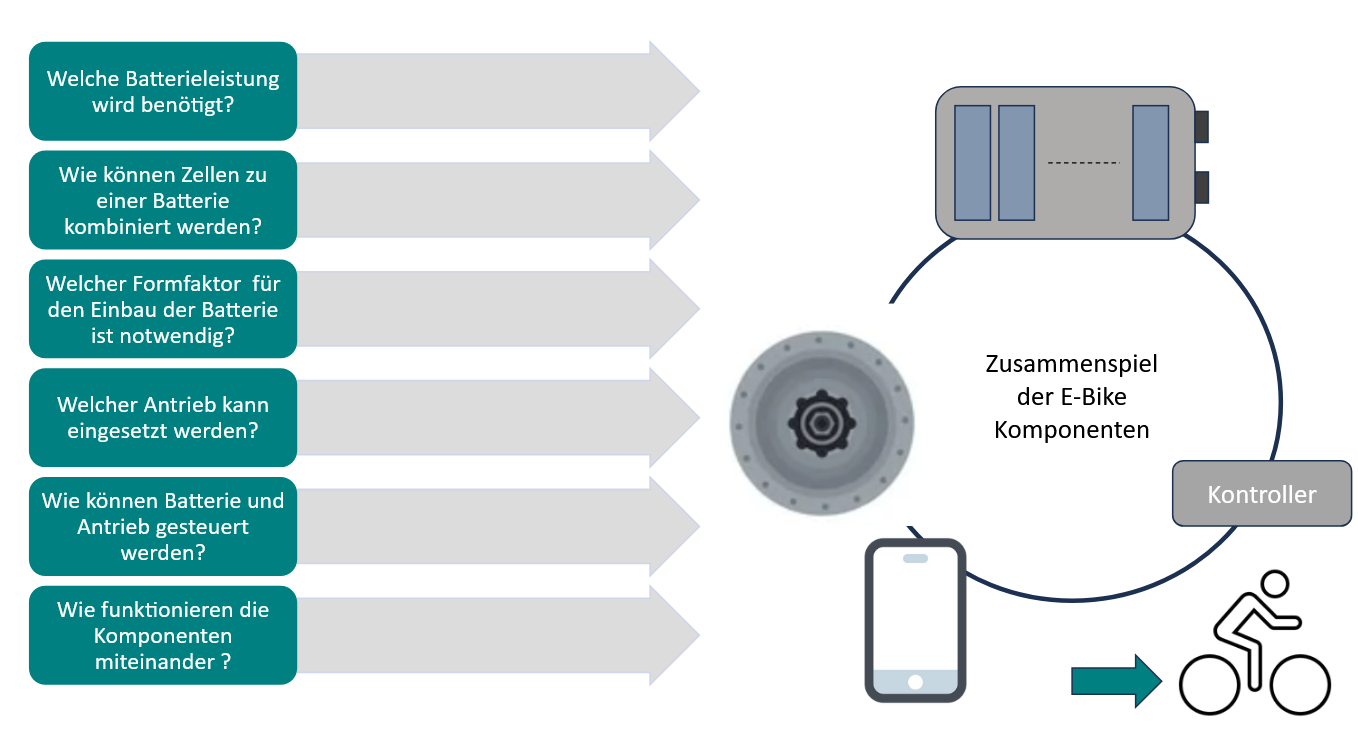
\includegraphics[width=11cm]{images/Flussdiagramm_E-bike.png}
    \caption{Zusammenspiel der E-Bike Komponenten}
    \label{fig:Komponenten}
\end{figure}


Diese wesentlichen Komponenten arbeiten zusammen, um ein E-Bike zu bilden, welches dem Fahrer elektrische Unterstützung beim Treten bietet und das Fahren erleichtert.